\subsubsection{Architektura programu}

V následující sekci budu používat obecný pojem \emph{modul} pro ohraničenou část
programu, implementující nějakou část funkcionality. Veřejné rozhraní modulu
definuje vstupní body, pomocí nichž s ním mohou ostatní moduly komunikovat.
Ty jsou zde reprezentovány funkcemi, makry a metodami, které modul poskytuje
a specifikacemi jejich parametrů. V Common Lispu sice tuto entitu nazýváme
\emph{package}, tento pojem se však špatně skloňuje a celkově narušuje plynulost
textu.

\begin{framed}
  Přesunout stylistické poznámky do zvlaštní sekce za úvod
\end{framed}

Obrázek \ref{modules} zobrazuje architekturu knihovny ExiL, tedy moduly, do
kterých je kód knihovny rozdělen a jejich vzájemnou komunikaci. Orientace šipek
určuje směr volání funkcí (metod, maker) poskytovaných moduly, např. modul
\verb|front-end| volá funkce modulu \verb|parser| a ne naopak. Těmito voláními
jsou zároveň definovány závislosti mezi moduly, ty mají tedy stejnou orientaci.

\begin{figure}[h]
\centering
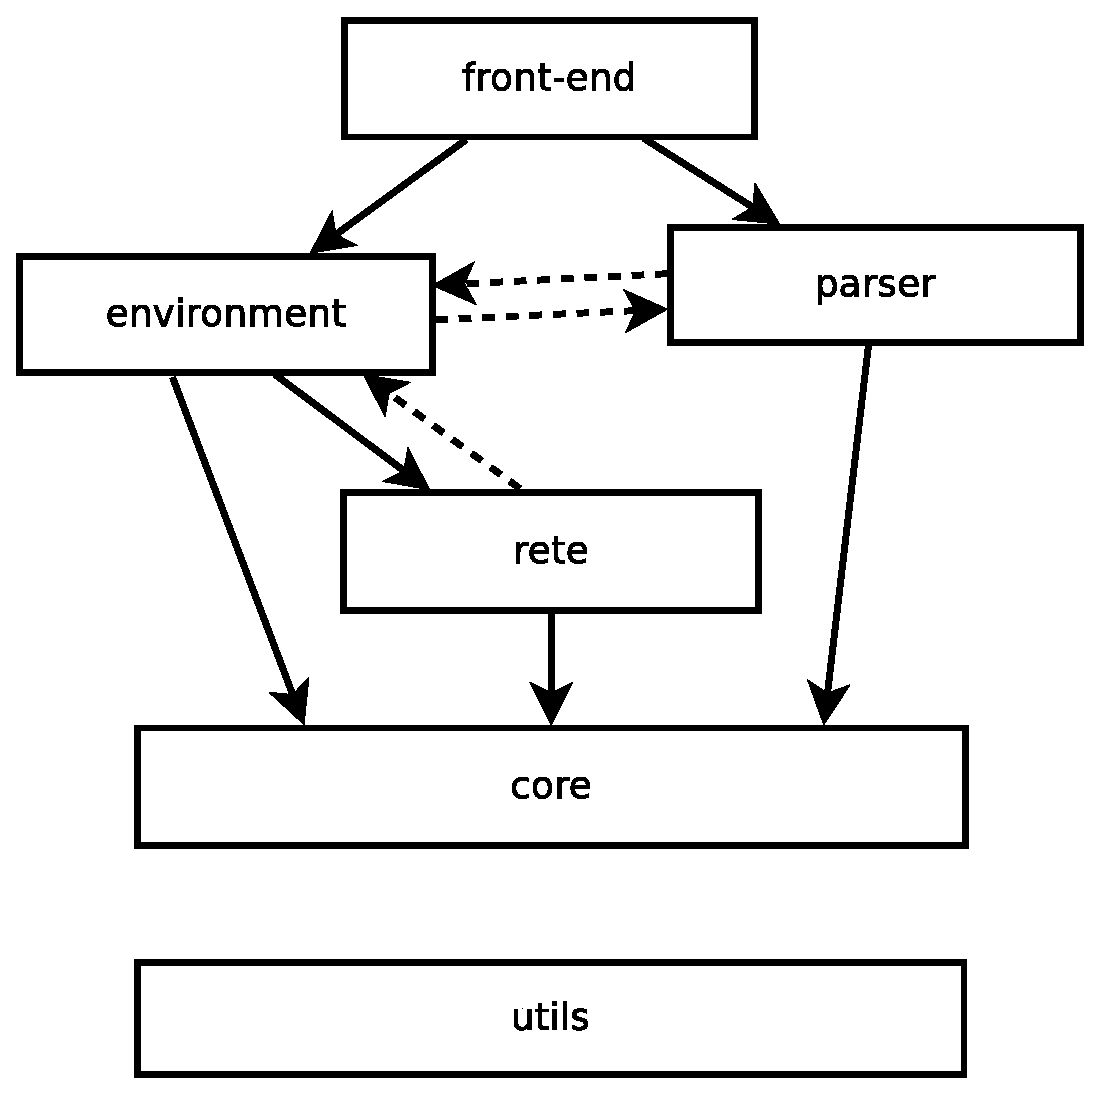
\includegraphics[height=10cm]{modules.eps}
\caption{Architektura ExiLu}
\label{modules}
\end{figure}

Modul \verb|utils| definuje různorodé pomocné funkce a makra, která jsou volána
všemi ostatními moduly. V obrázku \ref{modules} bych tedy mohl zahrnout šipky ze
všech ostatních modulů do modulu \verb|utils|, to by jej však činilo zbytečně
nepřehledným. Většina funkcí a maker, která modul definuje, usnadňuje
nízkoúrovňovou práci se symboly a datovými strukturami - (asociativními)
seznamy, množinami, stromy, \emph{hashovacími tabulkami} apod.

Modul \verb|core| definuje základní objekty, s nimiž zbytek knihovny
pracuje.  Ty reprezentují fakty, vzory, šablony a pravidla. Fakty a vzory jsou
definovány ve dvou variantách - jednoduché a strukturované (\emph{templated}),
jak jsem uvedl v uživatelské příručce.

% \begin{framed}
% Následující 4 odstavce jsou oproti zbytku příliš detailní. Odstranit minimálně
% konkrétní názvy objeků a metody (pokud to bude možné)
% \end{framed}

% Protože fakty a vzory sdílí velkou část funkcionality, definuje modul obecné
% objekty \verb|simple-object| a \verb|templated-object|, které implementují
% společnou funkcionalitu. Jednoduché a strukturované fakty a vzory jsou pak
% specializacemi těchto objektů.

% Objekty \verb|simple-object| a \verb|template-object| navíc dědí z objektu
% \verb|basic-object|. Hlavním úkolem tohoto objektu je smazat rozdíly mezi
% jednoduchými a strukturovanými objekty. To je zajištěno \emph{metodami}
% \verb|object-slot| a~\verb|atom-position|, které mají protichůdnou funkci.
% Metoda \verb|object-slot| bere objekt a pozici atomu (index seznamu u
% jednoduchého, název slotu u strukturovaného objektu) a vrací jeho hodnotu.
% Metoda \verb|atom-position| naopak bere objekt a hodnotu atomu a vrací jeho
% pozici (tedy index, nebo název slotu). Díky tomu může modul \verb|rete|
% porovnávat a vyhledávat jednotlivé atomy objektů, aniž by ho zajímalo, s jakým
% typem objektu zrovna pracuje.

% Každý typ \verb|core| objektu také implementuje \emph{predikát} ekvivalence,
% pomocí kterého je možno objekty vyhledávat v datových strukturách, udržovaných
% prostředím a uzly sítě RETE (viz dále) a to opět bez ohledu na konkrétní typ
% objektu.

% Modul \verb|core| také implementuje metodu \verb|match-against-pattern|, která
% umožňuje srovnání jednoho faktu se vzorem. Ta kromě \emph{booleovské} hodnoty,
% zda se objekty shodují, vrací v případě shody také použité vazby proměnných.
% Prostředí využívá tuto metodu při zpětné inferenci a při vyhodnocování důsledků
% pravidel.

% Modul \verb|rete| definuje objekt \verb|rete|, který reprezentuje síť RETE. Ta
Modul \verb|rete| implementuje algoritmus RETE, který slouží slouží k
efektivnímu vyhodnocování podmínek odvozovacích pravidel. Algoritmus je
implementován \emph{dataflow} sítí, jejíž fungování popíšu detailně v sekci
\ref{rete} Algoritmus RETE je sice nejkomplexnější částí ExiLu, veřejné rozhraní
modulu \verb|rete| je však velmi jednoduché.

Modul poskytuje dvojici metod kterými síť RETE upozorníme na přidání nebo
odebrání pravidel. Ty dle potřeby doplní síť o uzly potřebné k vyhodnocení
podmínek těchto pravidel, případně uzly při odebrání pravidla odstraní.

Další dvojice metod upozorní síť na přidání faktu do (resp. odebrání z) pracovní
paměti. Síť pak přepočítá splněné podmínky pravidel a případně upozorní
prostředí na nově přibyvší nebo rozbité shody (\emph{broken match} - pravidla,
která byla splněná a už nejsou).

Modul \verb|environment| definuje stejnojmenný objekt, který udržuje průbežný
stav prostředí a řídí průběh inference. Hodnoty, které stav prostředí tvoří,
jsem popsal v sekci \ref{env cleanup} Prostředí udržuje krom jiného
\emph{referenci} na síť \verb|rete|, kterou upozorňuje na nastalé změny.

Modul \verb|parser| zajišťuje vytváření \verb|core| objektů z externí
reprezentace (té, kterou předáváme makrům při práci s knihovnou). Modul
rozpoznává jak základní, tak CLIPSovou syntax, takže o to, kterou z nich
uživatel používá se zbytek kódu nemusí dále starat.

Při parsování strukturovaných faktů či vzorů se \verb|parser| dotazuje
aktuálního prostředí na definici šablony. Při zpětné inferenci prostředí
vyhodnocuje volání \verb|assert| v důsledcích pravidel a žádá \verb|parser| o
zparsování reprezentací faktů v~nich. Proto jsem mezi moduly \verb|environment|
a \verb|parser| přidal šrafované šipky. Kromě těchto nutných interakcí spolu
však moduly nekomunikují.

Modul \verb|front-end| udržuje seznam definovaných prostředí a ví, které je
právě aktivní. Kromě manipulace tohoto seznamu modul sám žádnou funkcionalitu
neimplementuje. Pouze quotuje parametry předané makrům, předává je
\verb|parser|u a výsledné objekty (se zbytkem parametrů) pak aktivnímu prostředí.

Do diagramu jsem nezahrnul modul \verb|gui|. Ten implementuje grafické
uživatelské rozhraní a poskytuje jedinou metodu - \verb|show-gui|. Rozhraní se
dotazuje prostředí, se kterým je svázáno, na hodnoty aktuálního stavu a je jím
upozorněno, pokud se tyto změní.
